% 原书 p.250–p.256（PDF p.258–p.264）
% >>> p258
下面的结果可以很容易地由 $E_N$ 的定义与命题 9.3.1 推出，但若直接从刚性轨迹 $R_N$ 的定义出发
则似乎难以得到。

\begin{wcor}{9.3.1}
设 $N_1\subset N_2$ 是 $M$ 中的开子集，则 $R_{N_1}\subset R_{N_2}$。
\end{wcor}

\begin{wproof}
若 $x\notin R_{N_2}$，则存在 $x$ 在 $M$ 中的一个邻域 $U_x$ 使得 $e(U_x,N_2)=0$。由于
$N_1\subset N_2$，故 $e(U_x,N_1)=0$。因此 $x\notin R_{N_1}$，这蕴涵
$R_{N_1}\subset R_{N_2}$。
\end{wproof}

这里给出命题 9.3.1 的证明。

\begin{wproof}[命题 9.3.1 的证明]
为证明 $E_N\subset R_N$，反设 $x\in E_N$ 但 $x\notin R_N$，则存在 $\varphi\in\mathrm{Stab}(N)$
使得 $\varphi(x)\notin N$。特别地，存在 $M$ 中包含 $x$ 的一个邻域 $U_x$，使得
$\varphi(U_x)\cap N=\varnothing$。此外，对任意 $\epsilon>0$，存在
$\psi_\epsilon\in\mathrm{Stab}(N)$ 使得 $\|\psi_\epsilon^{-1}\varphi\|<\epsilon$ 且
$\psi_\epsilon^{-1}(N)=N$。于是我们有
\begin{equation}
  \psi_\epsilon^{-1}\varphi(U_x)\cap\psi_\epsilon^{-1}(N)
  =\psi_\epsilon^{-1}\varphi(U_x)\cap N=\varnothing .
  \tag{9.26}
\end{equation}
注意 $\psi_\epsilon^{-1}\varphi\in\Ham(M,\omega)$，而在 (9.26) 中令 $\epsilon\to0$，我们得到
$e(U_x,N)=0$，由 (9.25) 这蕴涵 $x\notin E_N$。这与 $x\in E_N$ 矛盾。

另一个方向要复杂一些。任取 $x\in R_N$，若 $x$ 的每个邻域 $U$ 都完全落在 $N$ 中，则由定理 6.1.2
有 $e(U,N)\ge e(U)>0$。现在，假设存在 $x$ 在 $M$ 中的邻域 $U$ 同时也与 $M\setminus N$ 相交，
则存在一条道路 $\gamma$，使得 $\gamma(0)=x$ 且 $\gamma(1)\in M\setminus N$。这有助于构造一个
映射 $\varphi\in\Ham_U$，使得 $\varphi(x)\notin N$，从而 $\varphi(x)\notin R_N$。由于 $R_N$
在 $\varphi$ 的作用下不变，这蕴涵 $\varphi\notin\mathrm{Stab}(N)$。

因此，存在 $2\epsilon_0>0$，使得每个满足 $\psi(N)=\varphi(N)$ 的 $\psi\in\Ham(M,\omega)$ 都
服从 $\|\psi\|\ge2\epsilon_0$（否则，一列满足 $\psi_m(N)=\varphi(N)$ 且
$\|\psi_m\|<\frac1m$ 的 $\{\psi_m\}$ 将导致一列 $\{\psi_m^{-1}\varphi\}$ 在 Hofer 意义下收敛到
$\varphi$）。现在，对满足 $\theta(U)\cap(N)=\varnothing$ 的 $\theta\in\Ham(M,\omega)$，
$\theta\varphi^{-1}\theta^{-1}$ 的支撑在 $\theta(U)$ 中，故
$(\varphi\theta\varphi^{-1}\theta^{-1})(N)=\varphi(N)$。于是我们得到
\[
  2\epsilon_0\le\|\varphi\theta\varphi^{-1}\theta^{-1}\|
  \le\|\varphi\theta\varphi^{-1}\|+\|\theta\|=2\|\theta\|,
\]
这里我们用了与命题 6.1.2 的证明中相同的技巧。因此 $\|\theta\|\ge\epsilon_0>0$，从而
$x\in E_N$。
\end{wproof}
% [Tutor Note: 本页内容是 §9.3 的收尾，因跨页而落在本章（PDF p258）开头；它与 9.4 节无关，
% 阅读 9.4 时可先跳过。记号提示：$E_N$ 由 (9.25) 定义、$R_N$ 为刚性轨迹（定义 9.3.1），
% $\mathrm{Stab}(N)$ 为稳定化子 (9.21)，$\|\cdot\|$ 是 Hofer 范数（与
% $\|\cdot\|_{\mathrm{Hofer}}$ 同义）。证明中最后一步「与命题 6.1.2 的证明中相同的技巧」指
% 三角不等式配合共轭不变性 $\|\varphi\theta\varphi^{-1}\|=\|\theta\|$；原文未写出这一等式，
% 它是 Hofer 范数的共轭不变性（第 6.1 节）。]

\section{拉格朗日之间的距离（大尺度）（Distance Between Lagrangians, Large Scale）}

\begin{keytakeaways}
\begin{itemize}
  \item 几何图像：由 Hofer 范数诱导的 Chekanov--Hofer 度量 $\delta_{\mathrm{CH}}$ 使拉格朗日
        轨道空间 $\mathcal{O}(L)$ 成为度量空间，本节要问它「有多大」——直径是否有限、
        是否含有大尺度的平直部分。
  \item 数学工具：拟同态（quasi-morphism）及其缺陷 $D(q)$、Bavard 对偶性、以及
        Alexander 技巧把支撑在赤道附近的哈密顿函数「推」到赤道上。
  \item 本节结论：$(\mathbb{D}^2,\omega_{\mathrm{std}})$ 的赤道具有大尺度刚性：存在
        $\Phi:([0,\infty),|\cdot|)\hookrightarrow(\mathcal{O}(L),\delta_{\mathrm{CH}})$，
        满足双边估计 (定理 9.4.1 的简化版)；而 $\R^2$ 中的单位圆正相反，
        $\mathcal{O}(L)$ 的直径有限（练习 9.4.1）。
  \item 定量机制：$\delta_{\mathrm{CH}}$ 由下确界定义，故正下界必须借助拟同态这一「代数机器」；
        这是 $\delta_{\mathrm{CH}}$ 与普通度量之间最本质的差别。
\end{itemize}
\end{keytakeaways}

回忆上一节中，由 Hofer 范数 $\|\cdot\|_{\mathrm{Hofer}}$ 诱导的伪度量
$\delta_{\|\cdot\|}=\delta_{\|\cdot\|_{\mathrm{Hofer}}}$（如 (9.20) 所定义）在 $L\subset(M,\omega)$
为拉格朗日子流形时，于轨道空间 $\mathcal{O}(L)$ 上是非退化的（见注 9.3.1）。历史上，这一真正的

% >>> p259
度量被称为 \textbf{Chekanov--Hofer 度量}，记作 $\delta_{\mathrm{CH}}$。如此我们得到一个度量空间
$(\mathcal{O}(L),\delta_{\mathrm{CH}})$。就度量几何而言，这里有一个自然的问题。

\begin{wque}{9.4.1}
度量空间 $(\mathcal{O}(L),\delta_{\mathrm{CH}})$ 有多大？
\end{wque}

描述度量空间中「大尺度」几何现象有各种方式。例如，人们可以简单地问：这样的度量空间直径有限
还是无限？即便对这样简单的问题，对度量空间 $(\mathcal{O}(L),\delta_{\mathrm{CH}})$ 而言也并不
容易。事实上，这里是辛几何中一个著名的未解问题。

\begin{wque}{9.4.2}（公开问题）
取 $(M,\omega)=(S^2,\omega_{\mathrm{area}})$，$L$ 为 $S^2$ 的标准赤道，则
$\mathrm{diam}(\mathcal{O}(L),\delta_{\mathrm{CH}})=+\infty$ 与否尚不清楚！
\end{wque}

对其他一些（二维）情形，与问题 9.4.2 相应的问题的答案通常是肯定的。下面就是一个漂亮的例子。

\begin{wthm}{9.4.1}（[138] 中的定理 1，[202] 中的定理 1）
对闭圆盘 $(\mathbb{D}^2,\omega_{\mathrm{std}})$（视为 $\C$ 中的标准圆盘），取拉格朗日赤道
$L:=\mathbb{D}^2\cap\R$（其中 $\R$ 表示 $\C$ 的实部），度量空间
$(\mathcal{O}(L),\delta_{\mathrm{CH}})$ 具有如下性质：存在常数 $A,B>0$，使得存在一个嵌入
$\Phi:(C_c^{\infty}([0,1];\R),\|\cdot\|_\infty)\hookrightarrow
(\mathcal{O}(L),\delta_{\mathrm{CH}})$，满足
\[
  \frac1A\big(\|f-g\|_\infty-B\big)
  \le\delta_{\mathrm{CH}}(\Phi(f),\Phi(g))
  \le\|f-g\|_\infty
\]
对任意 $f,g\in C_c^{\infty}([0,1];\R)$ 成立。
\end{wthm}
% [Tutor Note: 这是本节的核心定量结论：$\Phi$ 是一个「大尺度」嵌入，即把
% $(C_c^\infty([0,1];\R),\|\cdot\|_\infty)$ 的无穷维仿射结构几乎等距地放进
% $(\mathcal{O}(L),\delta_{\mathrm{CH}})$。左端出现加性误差 $-B$（并非乘性误差），因此它只保证
% 「大范围」的刚性——对 $\|f-g\|_\infty$ 很小的元素对不提供信息，这是大尺度几何的标准特征。
% 另注：$\Phi$ 的定义域在定理中写作 $C_c^\infty([0,1];\R)$（紧支撑光滑函数），而证明中只用到
% $C_c([0,1];\R)$（连续紧支撑）；原文后文用 $f_r\in C_c([0,1];\R)$ 并加以光滑化，两处口径
% 略有出入，不影响结论。]

由于 $(\mathbb{D}^2,\omega_{\mathrm{std}})$ 是带边界的紧流形，轨道空间 $\mathcal{O}(L)$ 是通过
群 $\Ham_c(\mathbb{D}^2,\omega_{\mathrm{std}})$ 的作用来定义的，该群由那些能由逐时刻紧支撑
（在 $\mathrm{int}(\mathbb{D}^2)$ 内）的哈密顿函数生成的哈密顿微分同胚组成。

下面的练习给出了另一个例子，同样是二维情形，但其结论与定理 9.4.1 的结论形成尖锐对比。

\begin{wexer}{9.4.1}（[224] 中的第 9 节）
考虑单位圆
\[
  L:=\{(x,y)\in\R^2\mid x^2+y^2=1\}
\]
以及轨道空间 $\mathcal{O}(L)=\{\varphi(L)\mid\varphi\in\Ham_c(\R^2,\omega_{\mathrm{std}})\}$。
这里 $\Ham_c(\R^2,\omega_{\mathrm{std}})$ 由 $(\R^2,\omega_{\mathrm{std}})$ 上具有紧支撑的
哈密顿微分同胚组成。按下面的各小问，证明度量空间 $(\mathcal{O}(L),\delta_{\mathrm{CH}})$ 的
直径是有限的。
\begin{enumerate}[label=(\roman*)]
  \item 对任意两个不同的 $L_1,L_2\in\mathcal{O}(L)$，证明：对充分大的 $\kappa>0$，起点 $L$ 的
        一个平移，比如 $L(\kappa):=\{(x,y)\in\R^2\mid(x-\kappa)^2+y^2=1\}$，满足
        $\delta_{\mathrm{CH}}(L_1,L(\kappa))=\delta_{\mathrm{CH}}(L_2,L(\kappa))$。
  \item 设 $L_1\cap L=L_2\cap L=\varnothing$。证明：对上面 (a) 中得到的 $L(\kappa)$，存在道路
        $\gamma_1,\gamma_2$，使得 $\gamma_1$ 落在 $\R^2\setminus L_1$ 的无界连通分支中，
        $\gamma_2$ 落在 $\R^2\setminus L_2$ 的无界连通分支中，并且二者都在 $\R^2$ 中连接点
        $(1,0)\in L$ 与 $(\kappa-1,0)\in L(\kappa)$。
\end{enumerate}
\end{wexer}
% [Tutor Note: 原文疑误——第 (ii) 与小问 (iii) 中两次写「(a) above」，但本题的小问标号是
% (i)、(ii)、(iii)、(iv)，并无 (a)；按上下文均应为 (i)。译文保留原文的「(a)」并在此说明，
% 详见 review_ch09b.md。另注：$\Ham_c$ 的下标 $c$ 表示 compact support（紧支撑），与
% $\Ham(\R^2,\omega_{\mathrm{std}})$（不要求紧支撑）不同；本练习中 $\mathcal{O}(L)$ 只用
% 紧支撑哈密顿微分同胚，否则平移群会使度量退化。]

% >>> p260
\begin{enumerate}[label=(\roman*),start=3]
  \item 由上面的 (a) 推出：对 $i=1,2$ 有
        $\delta_{\mathrm{CH}}(L,L_i)=\delta_{\mathrm{CH}}(L(\kappa),L_i)$。这蕴涵：若两个不同的
        $L_1,L_2\in\mathcal{O}(L)$ 满足 $L_1\cap L=L_2\cap L=\varnothing$，则
        $\delta_{\mathrm{CH}}(L,L_1)=\delta_{\mathrm{CH}}(L,L_2)$。
  \item 证明：存在一个一致的常数 $C>0$，使得对任意 $L'\in\mathcal{O}(L)$ 都有
        $\delta_{\mathrm{CH}}(L,L')\le C$。这里 $C$ 与 $L'$ 无关。
\end{enumerate}

\begin{wrem}{9.4.1}
上面的练习 9.4.1 展示了一个相当罕见的情形：度量空间
$(\mathcal{O}(L),\delta_{\mathrm{CH}})$ \emph{不}具有大尺度几何现象。另一方面，定理 9.4.1
之所以困难，是因为 $\delta_{\mathrm{CH}}$ 是通过下确界定义的，因此要得到非平凡（正）的下界
需要某些机器。证明这类结果的标准工具是经由\emph{拟同态}（quasi-morphism，即「相差一个有界
误差的同态」）——其精确定义见定义 9.4.1。
\end{wrem}

为降低复杂度，我们将证明 [202] 中定理 1 的一个简化版本：存在常数 $A,B>0$，使得存在一个嵌入
$\Phi:([0,\infty),|\cdot|)\hookrightarrow(\mathcal{O}(L),\delta_{\mathrm{CH}})$，满足
\[
  \frac1A\big(|r-s|-B\big)\le\delta_{\mathrm{CH}}(\Phi(r),\Phi(s))
\]
对任意 $r,s\in[0,\infty)$ 成立。这通常正是困难的那个方向，它反映了度量空间
$(\mathcal{O}(L),\delta_{\mathrm{CH}})$ 所要求的大尺度几何性质。

事实上，$\Phi$ 的构造一点也不神秘：给定 $r\in\R$，先如下构造
$f_r\in C_c([0,1];\R)$：考虑如下函数
\[
  f_r(x)=
  \begin{cases}
    2rx & \text{若 } 0\le x\le\frac12,\\[1mm]
    -2r(x-1) & \text{若 } \frac12\le x\le1,
  \end{cases}
\]
并在 $x=0,0.5,1$ 附近将其磨光，就得到所需的函数。我们仍把它记作 $f_r$（见 图 9.8 的左图）。

接着考虑 $\varphi_{F_r}^1(L)\in\mathcal{O}(L)$，其中 $F_r(z):=f_r(\pi|z|^2)$ 对任意
$z\in\mathbb{D}^2$。这样由起点 $L$ 形变而来的拉格朗日子流形可以由图 9.8 的右图示意。

我们的目标是证明
\[
  \delta_{\mathrm{CH}}\big(\varphi_{F_r}^1(L),\varphi_{F_s}^1(L)\big)
  \ge\frac1A\big(|r-s|-B\big).
\]
由 Hofer 范数 $\|\cdot\|_{\mathrm{Hofer}}$ 的共轭不变性质，只需证明
\begin{equation}
  \delta_{\mathrm{CH}}\big(\varphi_{F_r}^1(L),L\big)\ge\frac1A(r-B),
  \tag{9.27}
\end{equation}
因为
$\delta_{\mathrm{CH}}(\varphi_{F_r}^1(L),\varphi_{F_s}^1(L))
=\delta_{\mathrm{CH}}(\varphi_{F_{r-s}}^1(L),L)$。解读 $\delta_{\mathrm{CH}}$ 的定义可知，
证明 (9.27) 等价于证明
\begin{equation}
  \|\psi\|_{\mathrm{Hofer}}\ge\frac1A(r-B)
  \tag{9.28}
\end{equation}
% [Tutor Note: 原文此处先写「给定 $r\in\R$」，而上面简化定理中要求的是 $r,s\in[0,\infty)$；
% 取 $r\ge0$ 是为保证 $f_r\ge0$、从而 $F_r$ 的流有明确定义的「高度」解释，$r<0$ 时论证仍成立
% 但需对称处理。另注：$\pi|z|^2$ 中的 $\pi$ 是圆周率常数（不是投影映射 $\pi$！），这与本节
% 后文出现的投影 $\pi:V\to\R^2$ 是同名不同物，阅读时须按上下文区分。]

% >>> p261
\begin{figure}[htbp]
  \centering
  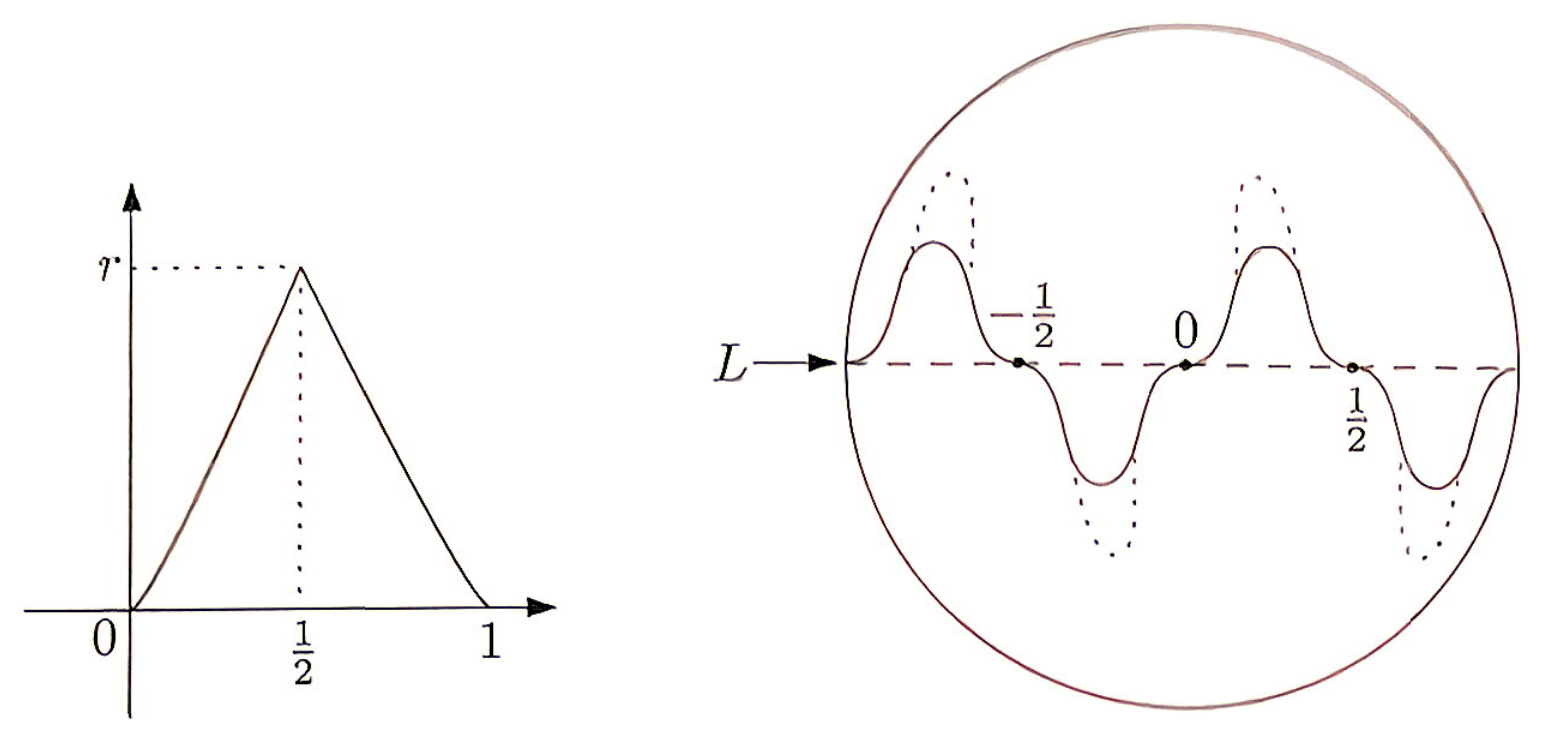
\includegraphics[width=0.82\linewidth]{figures/fig_p261_1.png}
  \caption*{图 9.8\quad $f_r$ 的图像（左）与形变后的赤道 $\varphi_{F_r}^1(L)$（右），
  位于 $(\mathbb{D}^2,\omega_{\mathrm{std}})$ 中（原书 p.253, Figure 9.8；PDF p.261）}
\end{figure}

其中 $\psi$ 取遍所有满足 $\psi(L)=\varphi_{F_r}^1(L)$ 的
$\psi\in\Ham_c(\mathbb{D}^2,\omega_{\mathrm{std}})$。特别地，
$\psi^{-1}\varphi_{F_r}^1\in\mathrm{Stab}(L)$，这里 $\mathrm{Stab}(L)$ 表示 (9.21) 中定义的
稳定化子，它是 $\Ham_c(\mathbb{D}^2,\omega_{\mathrm{std}})$ 的一个子群。

在给出证明之前，我们先绕道去讲拟同态。

\begin{wdefn}{9.4.1}
群 $G$ 上的一个\textbf{齐次拟同态}（homogeneous quasi-morphism）是一个函数 $q:G\to\R$，
使得对任意 $n\in\Z$ 有 $q(g^n)=nq(g)$，并且存在 $B\in\R_{\ge0}$ 使得
\[
  |q(ab)-q(a)-q(b)|\le B
\]
对任意 $a,b\in G$ 成立。这个常数 $B$ 通常称为 $q$ 的\textbf{缺陷}（defect），记作 $D(q)$。
\end{wdefn}

\begin{wexer}{9.4.2}
齐次拟同态 $q$ 在 $G$ 的任何阿贝尔子群上都是同态。此外，它对任意 $a,b\in G$ 满足
$q(bab^{-1})=q(a)$（换言之，齐次拟同态是一个\emph{类函数}）。
\end{wexer}

\begin{wexer}{9.4.3}
设 $q:G\to\R$ 为齐次拟同态，其缺陷记作 $D(q)$。(i) 证明：对任意换位子 $[a,b]\in G$，有
$|q([a,b])|\le D(q)$。(ii) 证明 (i) 中的关系是锐利的，即
\[
  \sup_{a,b}|q([a,b])|=D(q),
\]
其中上确界取遍所有 $a,b\in G$。（提示：先证明形如 $a^{2n}b^{2n}(ab)^{-2n}$ 的元素可以写成
$n$ 个换位子的乘积。）
\end{wexer}

\begin{wrem}{9.4.2}
这里还有另一个众所周知的结果，称为 \textbf{Bavard 对偶性}（Bavard's duality），它把
（稳定）换位子长度与拟同态联系起来：对任意 $x\in[G,G]$，有
\[
  \mathrm{scl}(x)=\sup\frac{|q(x)|}{D(q)},
\]
其中上确界取遍 $G$ 上所有\emph{不是}同态的齐次拟同态 $q$，而 $\mathrm{scl}$ 表示换位子长度
的齐次化（它确实是 $[G,G]$ 上一个共轭不变范数）。Bavard 对偶性的一个直接应用是探测
$\mathrm{scl}>0$（一般而言 $\mathrm{scl}$ 难以计算）——只需确认存在一个非平凡拟同态，而这
或多或少是一个构造性问题。
\end{wrem}

% >>> p262
给定群 $G$，$G$ 上非平凡拟同态的存在性是群论的中心问题之一。对辛几何中的某些群，我们可以基于
$G$ 自身的几何/动力学性质来构造（齐次）拟同态。下面的事实给出了一个例子。

\begin{wfact}{9.4.1}（[78] 中的定理 1.3）
在 $(\CP^1,\omega_{\mathrm{FS}})$ 上，存在齐次拟同态
$\mu:\Ham(\CP^1,\omega_{\mathrm{FS}})\to\R$，满足如下性质。
\begin{enumerate}[label=(\roman*)]
  \item 对任意 $\varphi\in\Ham(\CP^1,\omega_{\mathrm{FS}})$，有
        $|\mu(\varphi)|\le\|\varphi\|_{\mathrm{Hofer}}$。
  \item 给定哈密顿函数 $F:[0,1]\times M\to\R$，若
        $\bigcup_{t\in[0,1]}\mathrm{supp}(F_t)$ 是可位移的，则
    \begin{equation}
      \mu(\varphi_F^1)=\int_0^1\left(\int_{\CP^1}F\,\omega_{\mathrm{FS}}\right)\dd t .
      \tag{9.29}
    \end{equation}
        为简洁起见，用 $\mathrm{Cal}(F)$ 记 (9.29) 的右端。
  \item 把 $\CP^1$ 与 $S^2$ 等同。若对某个只依赖于时间 $t$ 的函数 $r(t)$ 有
        $F_t|_L=r(t)$，其中 $L$ 是 $S^2$ 的标准赤道，则
    \begin{equation}
      \mu(\varphi_F^1)=-\int_0^1r(t)\,\dd t+\mathrm{Cal}(F).
      \tag{9.30}
    \end{equation}
\end{enumerate}
\end{wfact}
% [Tutor Note: (ii) 中把哈密顿函数的定义域写成 $F:[0,1]\times M\to\R$，但本事实的流形是
% $\CP^1$，此处 $M$ 应为 $\CP^1$（原文沿用了第 1 章的通用记号 $M$），详见 review_ch09b.md。
% 另注「可位移的（displaceable）」：指存在 $\psi\in\Ham(M,\omega)$ 使
% $\psi(\bigcup_t\mathrm{supp}(F_t))\cap\bigcup_t\mathrm{supp}(F_t)=\varnothing$；
% 这是 Hofer 几何中「小支集」的标准技术假设，正是它保证 $\mathrm{Cal}(F)$ 只依赖
% $\varphi_F^1$ 而不依赖生成函数 $F$ 的选取。(9.29) 中的内层积分
% $\int_{\CP^1}F\omega_{\mathrm{FS}}$ 是 $F$ 在上同调基本类上的配对（按 (1.5) 的归一化，
% $\int_{\CP^1}\omega_{\mathrm{FS}}=\pi$）。]

注意 (9.29) 与 (9.30) 是两种罕见的情形——人们可以显式计算出一个拟同态的值。

借助事实 9.4.1 中的拟同态 $\mu$，我们就能给出定理 9.4.1 简化版本的证明，特别是给出不等式
(9.28)。

\begin{wproof}[简化版定理 9.4.1 的证明]
考虑嵌入 $\theta:\mathbb{D}^2(1/2)\hookrightarrow S^2(=\CP^1)$，由
$z\mapsto[\sqrt{1/2-|z|^2}:z]$ 给出；以及由下式定义的拟同态
$q:\Ham_c(\mathbb{D}^2,\omega_{\mathrm{std}})\to\R$：
\begin{equation}
  q(\varphi):=-\theta^*(\mu)+\mathrm{Cal}(\varphi),
  \tag{9.31}
\end{equation}
其中 $\theta^*(\mu)=\mu(\theta\circ\varphi\circ\theta^{-1})$。注意这里的
$\mathrm{Cal}(\varphi)\Big(=\mathrm{Cal}(\varphi_F^1)=\int_0^1\big(\int_{\mathbb{D}^2}
F\omega_{\mathrm{area}}\big)\dd t$，如 (9.29) 那样$\Big)$ 在时间 $1$ 映射上是良定义的
（而不只是在哈密顿函数层面）。事实上，这是一个深刻的事实——见考试 I 中的问题 A，其本质在于
我们的设定中 $\mathbb{D}^2$ 是恰当辛流形。

由事实 9.4.1 中的 (i)$\sim$(iii)，我们有下面几条观察。
% [Tutor Note: (9.31) 中 $\theta^*(\mu)$ 是拟同态 $\mu$ 沿嵌入 $\theta$ 的拉回，即
% $(\theta^*\mu)(\varphi)=\mu(\theta\varphi\theta^{-1})$；由于 $\theta$ 只把
% $\mathbb{D}^2(1/2)$ 放进 $S^2$，需先把 $\varphi$ 延拓到 $\mathbb{D}^2$ 之外（取恒等）才能
% 与 $\theta$ 复合，原文未明说这一点。$\mathrm{Cal}$ 的良定义性（只依赖 $\varphi_F^1$）是
% 本证明的关键，作者把它归于「考试 I 问题 A」，其标准证明用恰当辛流形上
% $\mathrm{Cal}$ 的同伦不变性（即 $\int_0^1\int_{\mathbb{D}^2}F_t\omega\dd t$ 不依赖生成
% $\varphi$ 的哈密顿函数选取）。]

% >>> p263
\begin{enumerate}[label=(\alph*)]
  \item 对任意 $\varphi\in\Ham_c(\mathbb{D}^2,\omega_{\mathrm{std}})$，事实 9.4.1 中的 (i) 与
        练习 9.4.2 蕴涵 $|q(\varphi)|\le A\cdot\|\varphi\|_{\mathrm{Hofer}}$，其中 $A>0$ 为
        某个常数。
  \item 对任意 $\varphi=\varphi_F^1$ 且 $F|_{|z|=\frac12}=r$，事实 9.4.1 中的 (iii) 蕴涵
        $q(\varphi)=r$，因为 $\theta$ 把 $\{z\in\mathbb{D}^2\mid|z|=1/2\}$ 映到 $S^2$ 的标准
        赤道。
  \item 我们还有 $|q(\psi^{-1}\varphi)+q(\psi)-q(\varphi)|\le B$，其中 $B>0$ 为某个常数
        （与 $\varphi,\psi\in\Ham_c(\mathbb{D}^2,\omega_{\mathrm{std}})$ 无关），$B$ 来自
        事实 9.4.1 中拟同态 $\mu$ 的缺陷 $D(\mu)$。事实上，映射
        $\mathrm{Cal}:\Ham_c(\mathbb{D}^2,\omega_{\mathrm{std}})\to\R$ 是同态（见考试 I 中
        问题 A 的 (b)）。换言之，$q$ 确实是 $\Ham_c(\mathbb{D}^2,\omega_{\mathrm{std}})$ 上的
        拟同态。
\end{enumerate}

上面三点蕴涵所需的结论 (9.28)。事实上，由上面的观察 (a)，我们有
$\|\psi\|_{\mathrm{Hofer}}\ge|q(\psi)|/A$。若 $q(\psi^{-1}\varphi_{F_r}^1)=0$，则由观察 (c)
我们有
\[
  \frac1A|q(\psi)|\ge\frac1A\big(q(\varphi_{F_r}^1)-B\big)=\frac1A(r-B),
\]
其中最后一步用了观察 (b)。因此，合并起来我们得到
$\|\psi\|_{\mathrm{Hofer}}\ge(r-B)/A$。

现在只剩下证明 $q(\psi^{-1}\varphi_{F_r}^1)=0$，这是上述论证中唯一的缺口。注意
$\psi^{-1}\varphi_{F_r}^1\in\mathrm{Stab}(L)$。事实上，我们将证明一个更一般的命题：
\begin{equation}
  q(\varphi)=0\qquad\text{对任意 }\varphi\in\mathrm{Stab}(L).
  \tag{9.32}
\end{equation}

下面是支持 (9.32) 的一个特殊情形：若 $\varphi=\varphi_F^1$，其中 $F|_U=0$（$U$ 为 $L$ 的
一个邻域），则由事实 9.4.1 中的 (iii) 本质上可得 $q(\varphi)=0$。然而，并非每个哈密顿函数
$F$ 都满足 $F|_L=0$，因此我们需要下面这个技巧（称为 \emph{Alexander 技巧}）：对任意
$s\in[\epsilon,1]$（其中 $\epsilon>0$ 充分小），如下映射
\[
  \psi_s(x):=
  \begin{cases}
    s\cdot\varphi_F^1\left(\dfrac xs\right) & \text{若 } |x|\le s,\\[2mm]
    x & \text{若 } |x|>s
  \end{cases}
\]
合起来定义了 $(\mathbb{D}^2,\omega_{\mathrm{std}})$ 上的一个\emph{哈密顿}微分同胚（见 [171]
中的推论 2.5.8），称为一个 \emph{Alexander 同痕}。然后考虑同痕
$\{\psi_s^{-1}\psi_{t(1-\epsilon)+\epsilon}\}_{t\in[0,1]}$，它是一族哈密顿微分同胚，连接
$\mathbf{1}$（$t=0$ 时）与 $\psi_s^{-1}\circ\varphi_F^1$（$t=1$ 时）。应用 Banyaga 的一个
结果（事实 6.1.1），我们得到
\[
  \{\psi_s^{-1}\psi_{t(1-\epsilon)+\epsilon}\}_{t\in[0,1]}
  =\{\varphi_H^t\}_{t\in[0,1]}
\]
其中 $H:[0,1]\times\mathbb{D}^2\to\R$ 为某个哈密顿函数。

现在，在 $t=1$ 处，我们可以把 $\varphi_F^1$ 重写成如下复合
\begin{equation}
  \varphi_F^1=\psi_\epsilon\circ\varphi_H^1,
  \tag{9.33}
\end{equation}
% [Tutor Note: Alexander 技巧的要点是：$\psi_s$ 在半径为 $s$ 的圆盘外是恒等、内部是把
% $\varphi_F^1$ 按因子 $s$ 缩小的结果，故其支撑可任意小。原文在此处前后记号略有不一致：
% 同痕族用参数 $s$，而 (9.33) 中直接用 $\psi_\epsilon$（即取 $s=\epsilon$），译文照原文排印。
% 另注意 (9.33) 的右端 $\varphi_H^1$ 的生成函数 $H$ 满足 $H|_L=0$，这正是下一步所需的，
% 而 $L$ 取赤道（$\mathbb{D}^2$ 边界的直线段）。]

% >>> p264
其中 $\psi_\epsilon$ 具有非常小的支撑，并且对赤道 $L$ 有 $H|_L=0$。第二个结论的理由是：
$\varphi_H^t(L)=L$ 对任意 $t\in[0,1]$ 成立蕴涵 $X_{H_t}$ 与 $L$ 相切，从而
$\dd H_t|_L=0$。于是 $H_t$ 在 $L$ 上为常数。又由于 $H_t$ 需具有紧支撑，我们得到
$H_t|_L=0$。

最后，由 (9.33) 的分解与定义 9.4.1，我们有
\[
  |q(\varphi)-q(\psi_\epsilon)-q(\varphi_H^1)|\le B .
\]
和 $q(\psi_\epsilon)+q(\varphi_H^1)$ 是 $\epsilon$-小的。事实上，$q(\psi_\epsilon)=0$，因为
$\mathrm{supp}(\psi_\epsilon)$ 是 $\epsilon$-小的；而 $q(\varphi_H^1)=0$，因为 $H|_L=0$
（再加上把观察 (b) 应用于 $\theta(L)\subset S^2$ 的闭包，那是 $S^2$ 的另一个标准赤道）。
因此 $|q(\varphi)|$ 被 $B$ 所逼近，特别地 $|q(\varphi)|\le2B$。又因 $q$ 是齐次拟同态（因为
事实 9.4.1 中的 $\mu$ 是齐次的，而 (9.31) 中的 $\mathrm{Cal}$ 是同态，故显然是齐次的），
通过考虑 $\varphi$ 的迭代，我们得到
\[
  n|q(\varphi)|=|q(\varphi^n)|\le2B .
\]
令 $n\to\infty$ 即得 $q(\varphi)=0$。
\end{wproof}
% [Tutor Note: 这段收尾有两点易错。其一，$q(\psi_\epsilon)=0$ 用的是 $\psi_\epsilon$ 的支撑
% 极小、从而落在某个与赤道不交的小圆盘内，于是由 (9.29) 的 $\mathrm{Cal}$ 公式与 (iii) 得
% $q=0$；原文只说「$\epsilon$-small」，实际含义是支撑落在 $\mathbb{D}^2$ 的一个充分小的
% 子圆盘内。其二，最后一步从 $n|q(\varphi)|\le 2B$ 推出 $q(\varphi)=0$，用的是
% $q(\varphi^n)=nq(\varphi)$（齐次性）以及 $n$ 可任意大——这是拟同态理论中的标准
% 「迭代消去」技巧。原文把「齐次（homogeneous）」拼作「homogenous」，属拼写笔误。]
